\documentclass[17pt]{memoir}

\title{Lessons for the Triduum}
\author{Compiled by Fr. G.R. Barnes}
\date{}


\usepackage{chant}

\usepackage[latin]{babel}
% \usepackage{microtype} % use this for the final render
\usepackage{fontspec}
\setmainfont{Minion3}

\usepackage{graphicx}
\graphicspath{ {./images/} }

\usepackage[lines=4]{lettrine}
\usepackage{Royal}
\renewcommand\LettrineFontHook{\Royal}

\usepackage{import}

\linespread{1.5}

\newcommand\flex{\dagger\ }
\newcommand\fullstop{\star\ }
\newcommand\question{ \ddagger}

\newcommand\reference[1]{\red{\hfill\small #1}}

\newcommand\triduumDay[1]{
    \newpage
    \begin{center}
        \scshape\HUGE
        #1
    \end{center}
}

\newcommand\lesson[1]{
    \newpage
    \begin{center}
        \red{Lectio #1}\bfseries
    \end{center}
    % \vfill
}

\pagenumbering{gobble}

\begin{document}

\triduumDay{Feria V in Cena Domini}

\vfill

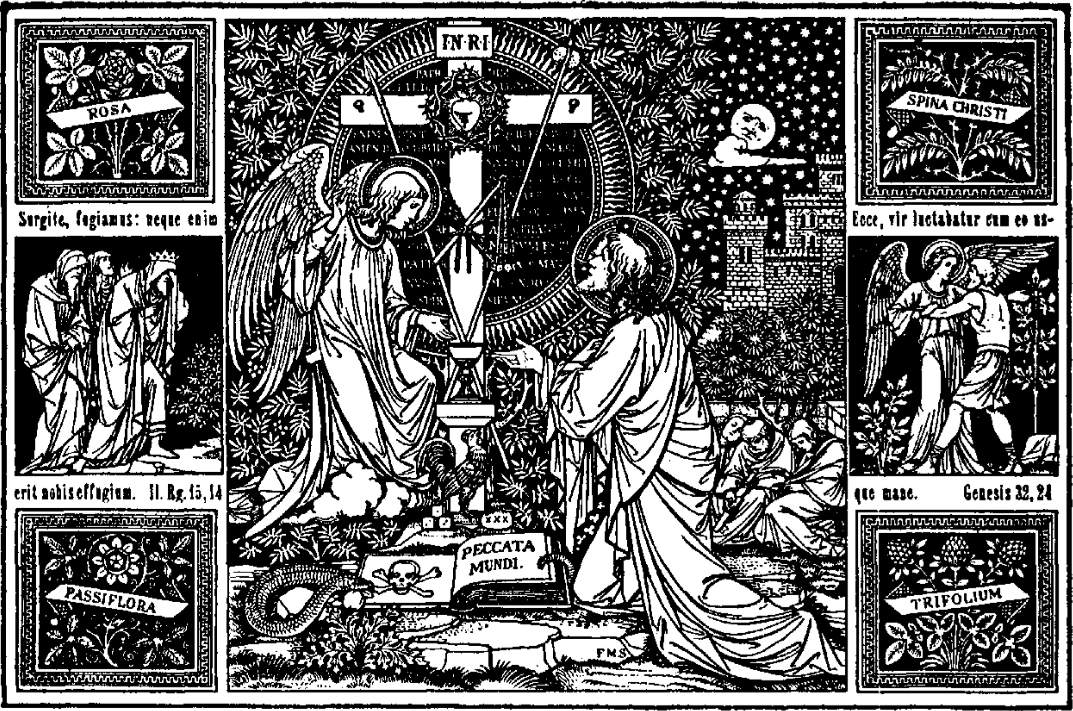
\includegraphics[width=\textwidth]{Thursday.jpg}

\vfill

\lesson{I}

\gregorioscore[a]{thursday_i}

\lesson{II}

\gregorioscore[a]{thursday_ii}

\lesson{III}

\gregorioscore[a]{thursday_iii}

\lesson{IV}
\lesson{V}
\lesson{VI}

\lesson{VII}

\noindent De Epístola prima beáti Pauli Apóstoli ad Corín\textbf{thi}os.$\star$

\reference{Cap. 11, 17-34}

\lettrine{H}{oc} autem præcí\textbf{pi}o:\flex non laudans quod non in mélius,
sed in detérius convení\textbf{tis.}\fullstop Primum quidem conveniéntibus
vobis in Ecclésiam, áudio scissúras esse inter vos, et ex parte
cre\textbf{do.}\fullstop Nam opórtet et hǽreses esse, ut et qui probáti sunt,
manifésti fiant in vo\textbf{bis.}\fullstop Conveniéntibus ergo vobis in unum,
jam non est Domínicam cenam manducá\textbf{re.}\fullstop Unusquísque enim suam
cenam præsúmit ad manducándum. Et álius quidem ésurit, álius autem ébrius
\textbf{est.}\fullstop \question Numquid domos non habétis ad manducándum et
\textit{bi}\textbf{béndum}? \question aut Ecclésiam Dei contémnitis, et
confúnditis eos,\question qui \textit{non} \textbf{habent}? \question Quid
di\textit{cam} \textbf{vobis}? \question \textit{Lau}\textbf{do vos}? In
\textbf{hoc} non \textbf{lau}do.\flex

\vfill

\lesson{VIII}

\lettrine{E}{go} enim accépi a Domino, quod et trádidi vobis, quóniam Dóminus
Jesus, in qua nocte tradebátur, accépit panem, et grátias agens fregit, et
dixit: Accípite et manducá\textbf{te}:\flex hoc est corpus meum, quod pro vobis
tradé\textbf{tur}:\flex hoc fácite in meam commemoratión\textbf{em}.\fullstop
Simíliter et cálicem, postquam cenávit, dicens: Hic calix novum Testaméntum est
in meo sán\textbf{gui}ne;\flex hoc fácite, quotiescúmque bibétis, in meam
commemorati\textbf{ón}em.\fullstop Quotiescúmque enim manducábitis panem hunc,
et cálicem bibétis, mortem Dómini annuntiábitis, \textbf{do}nec
\textbf{vé}niat.\flex

\vfill

\lesson{IX}

\lettrine{I}{taque} quicúmque manducáverit panem hunc, vel bíberit cálicem
Dómini indígne, reus erit córporis et sánguinis Dó\textbf{mi}ni.\fullstop
Probet autem seípsum ho\textbf{mo}:\flex et sic de pane illo edat, et de cálice
bi\textbf{bat}.\fullstop Qui enim mandúcat et bibit indígne, judícium sibi
mandúcat et bibit, non dijúdicans corpus Dó\textbf{mi}ni.\fullstop Ideo inter
vos multi infírmi et imbecílles, et dórmiunt mul\textbf{ti}.\fullstop Quod, si
nosmetípsos dijudicarémus, non útique judicaré\textbf{mur}.\fullstop Dum
judicámur autem, a Dómino corrípimur, ut non cum hoc mundo
damné\textbf{mur}.\fullstop Itaque, fratres mei, cum convenítis ad manducándum,
ínvicem exspectá\textbf{te}.\fullstop Si quis ésurit, domi
mandú\textbf{cet}:\flex ut non in judícium conveniá\textbf{tis}.\fullstop
Cétera autem, cum véne\textbf{ro}, dis\textbf{pó}nam.\flex

\vfill

\triduumDay{Feria VI in Parasceve}

\vfill

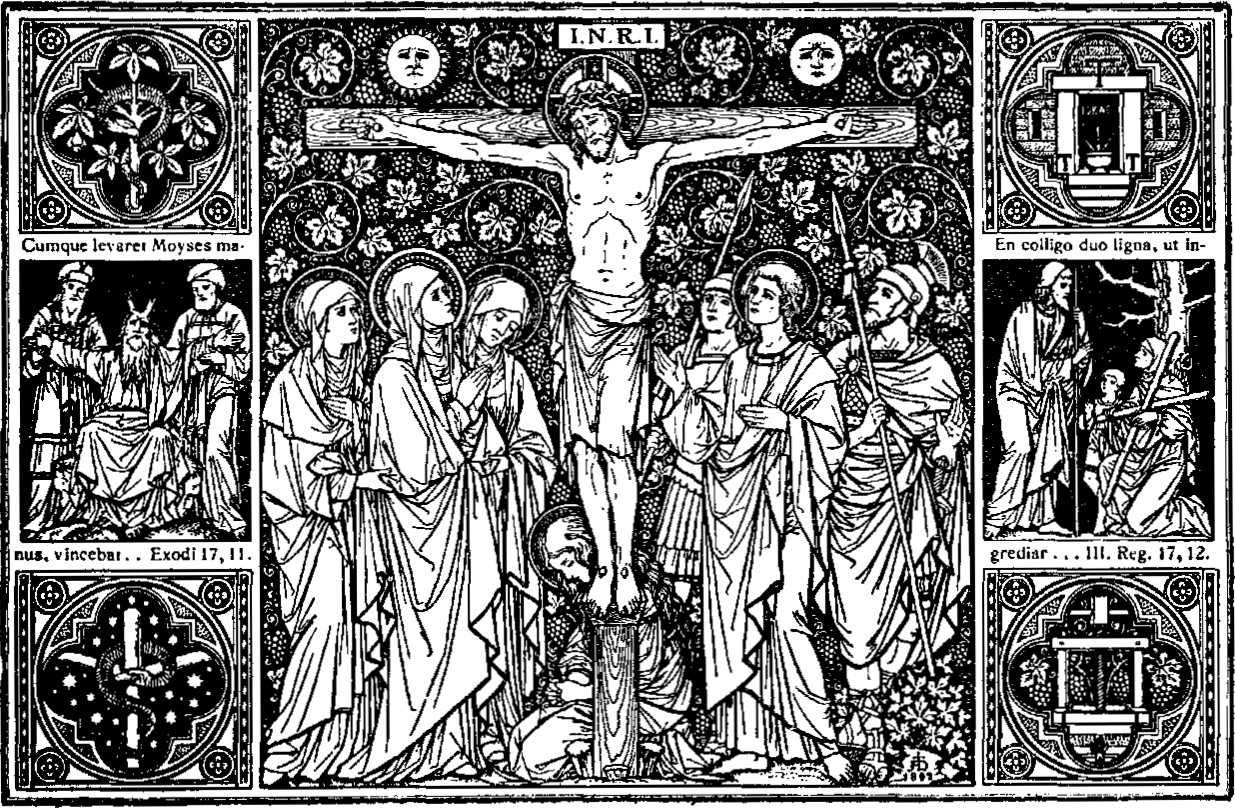
\includegraphics[width=\textwidth]{Friday.jpg}

\vfill

\lesson{I}

\lesson{II}
\lesson{III}
\lesson{IV}
\lesson{V}
\lesson{VI}

\lesson{VII}

\noindent De Epístola beáti Pauli Apóstoli ad Hebr\'æ\textbf{os}\flex

\reference{Cap. 4, 11-15}

\lettrine{F}{estinémus} íngredi in illam réqui\textbf{em}:\flex ut ne in
idípsum quis íncidat incredulitátis exém\textbf{plum}.\fullstop Vivus est enim
sermo Dei, et éfficax, et penetrabílior omni gládio ancí\textbf{pi}ti:\flex et
pertíngens usque ad divisiónem ánimæ ac spíritus, compágum quoque ae
medullárum, et discrétor cogitatiónum et intentiónum cor\textbf{dis}.\fullstop
Et non est ulla creatúra invisíbilis in conspéctu e\textbf{jus}:\flex ómnia
autem nuda et apérta sunt óculis ejus, ad quern nobis ser\textbf{mo}.\fullstop
Habéntes ergo Pontíficem magnum,qui penetrávit cælos, Jesum, Fílium
De\textbf{i}:\flex teneámus confessió\textbf{nem}.\fullstop Non enim habémus
Pontíficem, qui non possit cómpati infírmitátíbus nos\textbf{trís}:\flex
tentátum autem per ómnia pro similitúdine \textbf{abs}que
pec\textbf{cá}to.\flex

\vfill

\lesson{VIII}

\lettrine{A}{deámus} ergo cum fidúcia ad thronum grá\textbf{ti}æ:\flex ut
misericórdiam consequámur, et grátiam inveniámus in auxílio
opportú\textbf{no}.\fullstop Omnis namque Póntifex ex nomínibus assúmptus, pro
homínibus constitute in iis, quæ sunt ad Deum, ut ófferat dona et sacrifícia
pro peccá\textbf{tis}:\flex qui condolére possit iis, qui ignorant et
er\textbf{rant}:\flex quóniam et ipse circúmdatus est
infirmitá\textbf{te}:\flex et proptérea debet quemádmodum pro pópulo, ita étiam
et pro semetípso offérre \textbf{pro} pec\textbf{cá}tis.\flex

\vfill

\lesson{IX}

\lettrine{N}{ec} quisquam sumit sibi honórem, sed qui vocátur a Deo, tamquam
A\textbf{ar}on.\fullstop Sic et Christus non semetípsum clarificávit ut
Póntifex fí\textbf{er}et:\flex sed qui locútus est ad eum: Fílius meus es tu, ego hódie génui
\textbf{te}.\fullstop Quemádmodum et in álio loco dicit: Tu es sacérdos in ætérnum, secúndum
órdinem Melchí\textbf{se}dech.\fullstop Qui in diébus carnis suæ, preces supplicationésque ad
eum, qui possit ilium salvum fácere a morte, cum clamóre válido et lácrimis
ófferens, exaudítus est pro sua reverén\textbf{ti}a.\fullstop Et quidem cum esset Fílius Dei,
dídicit, ex iis, quæ passus est, obœdién\textbf{ti}am:\flex et consummátus, factus est
omnibus obtemperántibus sibi causa salútis ætérnæ, appellátus a Deo Póntifex
juxta órdi\textbf{nem} Mel\textbf{chí}sedech.\flex

\triduumDay{Sabbato Sancto}

\vfill

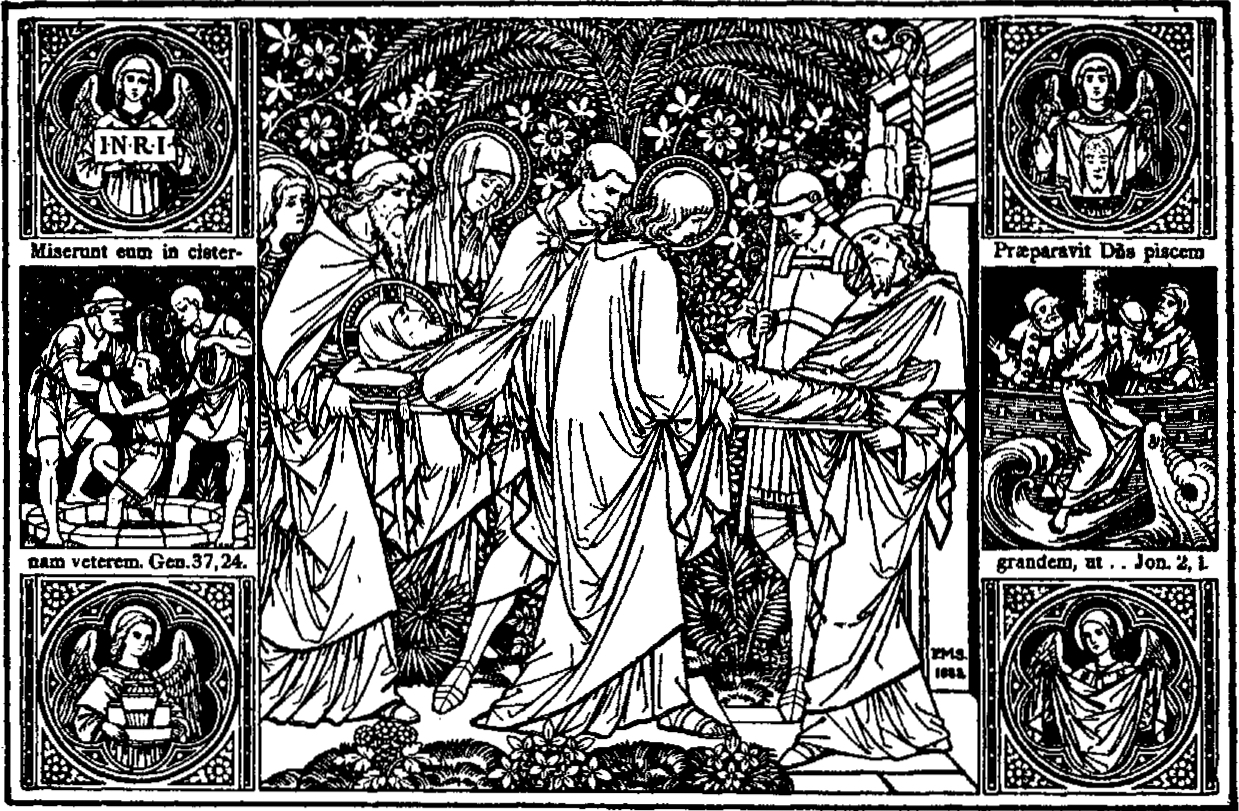
\includegraphics[width=\textwidth]{Saturday.jpg}

\vfill

\lesson{I}


\lesson{II}

\lesson{III}

\reference{Lam 5:1-11}

\gregorioscore[a]{saturday_iii}

\lesson{IV}
\lesson{V}
\lesson{VI}

\lesson{VII}

\noindent De Epístola beáti Pauli Apóstoli ad Hebr\'æ\textbf{os}\fullstop

\reference{Cap. 9, 11-22}

\lettrine{C}{hristus} assístens Póntifex futurórum bonórum, per ámplius et
perféctius tabernáculum non manufáctum, id est, non hujus
creatíón\textbf{is}:\flex neque per sánguinem hircórum aut vitulórum, sed per
próprium sánguinem introívit semel in Sancta, ætérna redemptióne
invén\textbf{ta}.\fullstop Si enim sanguis hircórum et taurórum et cinis vítulæ
aspérsus inquinátos sanctíficat ad emundatiónem car\textbf{nis}:\flex quanto
magis sanguis Christi, qui per Spíritum Sanctum semetípsum óbtulit immaculátum
Deo, emundábit consciéntiam nostram ab opéribus mórtuis, ad serviéndum
\textbf{De}o vi\textbf{vén}ti?\flex

\vfill

\lesson{VIII}

\lettrine{E}{t} ídeo novi Testaménti mediá\textbf{tor} est:\flex ut, morte
intercedénte, in redemptiónem eárum prævaricatiónum, quæ erant sub priori
Testaménto, repromissiónem accípiant, qui vocáti sunt ætérnæ
hereditá\textbf{tis}.\fullstop Ubi enim testamén\textbf{tum} est:\flex mors
necésse est intercédat testató\textbf{ris}.\fullstop Testaméntum enim in
mórtuis confirmá\textbf{tum} est:\flex alióquin nondum valet, dum vivit, qui
testá\textbf{tus} est.\fullstop Unde nec primum quidem sine sanguine
\textbf{de}di\textbf{cá}tum est.\flex

\vfill

\lesson{IX}

\lettrine{L}{ecto} enim omni mandáto Legis a Móyse univérso
pó\textbf{pu}lo:\flex accípiens sánguinem vitulórum et hircórum cum aqua et
lana coccínea et hyssó\textbf{po}:\flex ipsum quoque librum et omnem pópulum
aspérsit, dicens: Hic sanguis Testaménti, quod mandávit ad vos
De\textbf{us}.\fullstop Etiam tabernáculum et ómnia vasa ministérii sanguine
simíliter aspér\textbf{sit}:\flex et ómnia pæne in sanguine secúndum legem
mundán\textbf{tur}:\flex et sine sánguinis effusióne non \textbf{fit}
re\textbf{mís}sio.\flex

\vfill

\end{document}
